\documentclass{article}          
\usepackage{tikz}
\usetikzlibrary{positioning,shapes,fit,arrows}
\pagestyle{empty}

\definecolor{myblue}{RGB}{56,94,141}
\begin{document}

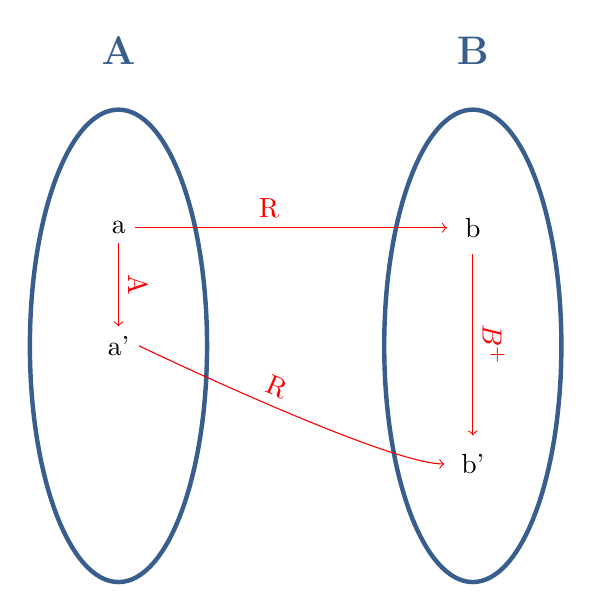
\begin{tikzpicture}[scale=.75]
\draw[ultra thick,myblue] (0,0) circle [x radius=1.5cm, y radius=4cm]
                    (6,0) circle [x radius=1.5cm, y radius=4cm];
                    
\node[font=\color{myblue}\Large\bfseries] at (0,5) {A};
\node[font=\color{myblue}\Large\bfseries] at (6,5) {B};  

\node (a1)  at (0,2)  {a};
\node (a2) at (0,0)   {a'};
%"\node (aux1) at (3,2)  {};

\node[circle] (b1) at (6,2)  {b}; 
\node[circle] (b2) at (6,-2)  {b'};


% \draw[thick,->,myblue] (b1) -- (b2);
% \draw[thick,->,myblue] (a1.east) -- (b1);
\draw[->,red] (a1.east) .. controls +(up:0cm) and +(left:1cm) .. node[above,sloped] {R} (b1.west);
\draw[->,red] (a2.east) .. controls +(up:0cm) and +(left:1cm) .. node[above,sloped] {R} (b2.west);
\draw[->,red] (a1.south) .. controls +(up:0cm) and +(left:0cm) .. node[above,sloped] {A} (a2.north);
\draw[->,red] (b1.south) .. controls +(up:0cm) and +(left:0cm) .. node[above,sloped] {$B^+$} (b2.north);
% \draw[thick,->,myblue] (a2.east) -- (b2);
% Referências: https://en.wikibooks.org/wiki/LaTeX/PGF/TikZ

\end{tikzpicture}

\end{document}